\documentclass[11pt]{article}
\usepackage{amsmath, amssymb, amsthm}
\usepackage{geometry}
\usepackage{graphicx}
\geometry{margin=1in}
\setlength{\parindent}{0pt} 
\title{Foundations of Machine Learning -- Lecture 6 Notes}
\author{}
\date{}

\begin{document}
\maketitle

\section*{Nearest Neighbor Classifier}
This is a non-parametric model, meaning the model does not assume a fixed functional form.
The model grows in complexity as data grows and the number of parameters is not fixed.
This makes the model very flexible with essentially no training step.
However, it requires large amounts of data and is slow during inference.

\begin{itemize}
	\item \textbf{Learning step:} Store all training examples (samples and labels).
	\item \textbf{Prediction step:} To classify a new example $x$, find the closest sample $x^{(i)}$ in the training set with some distance function d, such that:
	      \[
		      d(x, x^{(i)}) < d(x, x^{(j)}) \quad \forall j \neq i
	      \]
	      Then assign the class:
	      \[
		      y = y^{(i)}
	      \]
\end{itemize}

\section*{K-Nearest Neighbor (KNN) Classifier}
This is a generalization of the Nearest Neighbor classifier.
Instead of looking at only one neighbor, the algorithm considers the $K$ closest training examples.

\begin{itemize}
	\item \textbf{Learning step:} Store all training examples (samples and labels).
	\item \textbf{Prediction step:} To classify a new example $x$, find the set of $K$ closest samples:
	      \[
		      X_K = \{ x^{(\pi(k))} \}_{k=1}^K
	      \]
	      such that
	      \[
		      d(x, x^{(i)}) < d(x, x^{(j)}) \quad \forall x^{(i)} \in X_K, \ \forall x^{(j)} \notin X_K
	      \]
	      Then assign $x$ to the most frequent class among its $K$ nearest neighbors.
\end{itemize}

\begin{figure}[ht!]
	\centering
	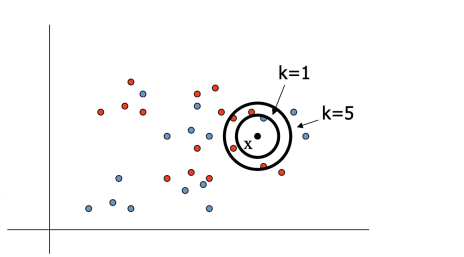
\includegraphics[width=0.5\textwidth]{../imgs/knn.png} % 
	\caption{KNN boundry example}
\end{figure}


\subsection*{How to Find Distance}
The performance of KNN depends on two design choices: the distance metric and the value of $K$.

A common way to find the distance is the Minkowski distance of order $p \geq 1$:
\[
	d_p(u, v) = \left( \sum_i |u_i - v_i|^p \right)^{\tfrac{1}{p}}
\]
\begin{itemize}
	\item $p = 2$: Euclidean distance, $d_2(u,v) = \|u - v\|$ \\
	      \textit{Interpretation:} shortest line between two points.
	\item $p = 1$: Manhattan distance, $d_1(u,v) = \sum_i |u_i - v_i|$ \\
	      \textit{Interpretation:} sum of coordinate steps (like moving on a grid).
	\item $p = \infty$: Chebyshev distance, $d_\infty(u,v) = \max_i |u_i - v_i|$ \\
	      \textit{Interpretation:} the biggest single-step difference dominates.
\end{itemize}

\subsection*{Choosing $K$}

There is no universal formula to determine the best $K$.
A common approach is to start with candidate $K$ values and evaluate performance.
\begin{itemize}
	\item Small $K$: prone to overfitting, sensitive to noise.
	\item Large $K$: smoother but may underfit, blurring class distinctions.
\end{itemize}


\section*{The Curse of dimensionality}
There is a major pitfall when it comes to KNN models with higher dimensional data.
Exponential growth in the number of examples is required to maintain a given sampling density.
Meaning our distances lose their meaning in higher dimensions.

\begin{figure}[ht!]
	\centering
	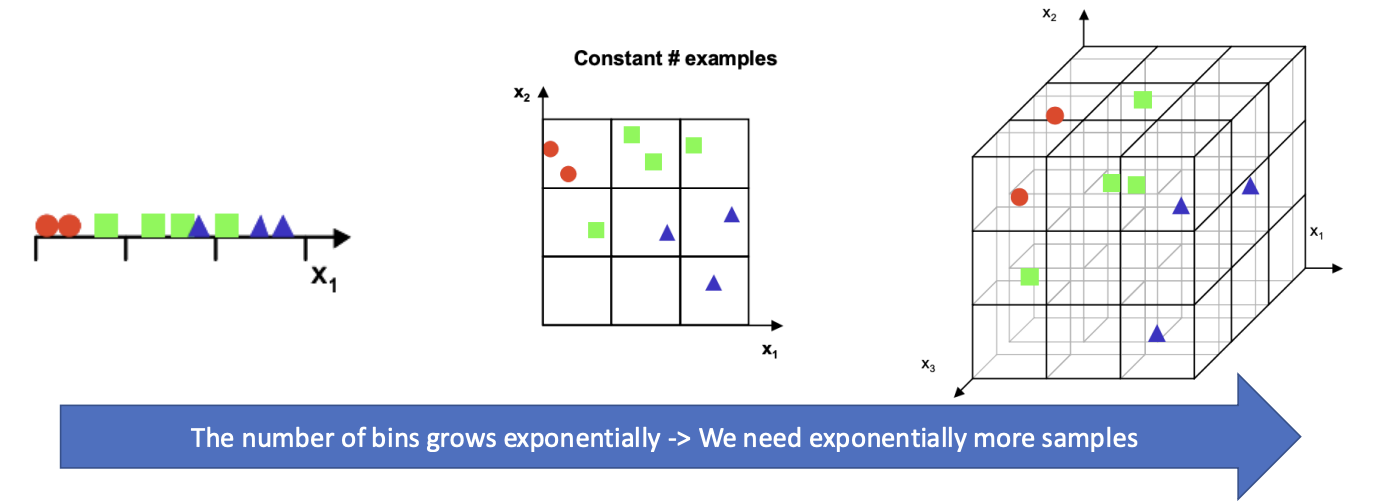
\includegraphics[width=0.5\textwidth]{../imgs/knn-dims.png} % 
	\caption{KNN Sparsity}
\end{figure}

In high dimensional spaces data becomes more sparce.

The concept of proximity or the neasrst point loses its usefulness and becomes less meaningful
as we increase the number of dimensions.

As the number of dimensions increases toward infinity, the ratio between the distance to the farthest point and the distance to the nearest point approaches 1. In this case, the nearest neighbor problem becomes poorly defined.

As a rule of thumb, for very high dimensional a lower norm metric, like the Manhattan (1 Norm)
probably behaves better than higher norm metrics.


\section*{KNN Regression}
\textbf{TODO}

\section*{Computational complexity}
The computational complexity of KNN with a training dataset of $N$ samples in a d-dimensional space is $O(dN)$

But we can use method to reduce this complexity...
\paragraph{Approximate nearest neighbor methods}
This involves giving up exactness and instead finding a neighbor that is “good enough.” This allows us to use structures like trees, hashing, or graphs to avoid scanning the entire dataset, cutting computational complexity.

\paragraph{Locality Sensitive Hashing}
LSH leverages the power of hash functions to transform data points into hash codes, facilitating faster and approximate similarity searches.

Hash functions are carefully crafted to map high-dimensional data points into hash codes. These codes are constructed in a way that similar points in the original space are likely to share the same or nearby hash codes.



\end{document}
